\documentclass{article}
\usepackage{amsmath,amssymb}
\usepackage{graphicx,color}
\usepackage{gensymb}

\title{\bf{Mid-Project Review: C++ implementation of the Metropolis-Hasting Algorithm}}
\author{Nicholas Malaya \\ University of Texas at Austin} \date{}

\begin{document}
\maketitle

\section{Introduction}

Bayesian Inference is a powerful statistical method that has found a
variety of applications in uncertainty quantification, decision theory,
model selection and many others. These methods have been applied to
diverse fields such as epidemiology, spam filters, computer vision, as
well as assessments of the reliability of the readyness of the United
States nuclear weapon stockpiles.  

However, Bayes' Theorem, despite existing since the 18th century, has
only recently become more prevalent in scientific applications. The
recent dramatic growth in Bayesian methods coincides with the
exponential expansion of computational power. This is because for all
but a small set of models, the posterior distribution is unable to be
analytically determined, and must be statistically sampled, often
requiring far more samples than are humanly possible to generate. 

For this project, we have developed a C++ implementation of the
Metropolis-Hastings algorithm. This is a Markov Chain Monte Carlo (MCMC)
method to sample from a probability distribution.  These samples will be
generated in order to estimate the posterior of a distribution for a
Bayesian Inference problem. We will generate results for a few different
models, in order to investigate the model against a known (analytic)
conjugate prior, as well as more complicated (non-tracible without
sampling) distributions.   

The code is written in C++, and will be parallelized with openMP. 
\section{Methodology}
%
% 3-4 page report on the progess of the project 
%

Suppose we have a posterior that we want to sample from, but:
\begin{itemize}
 \item the posterior doesn't look like any distribution we know (no
       conjugate model exists)
 \item some (or all) of the full conditionals do not look like any
      distributions we know (no Gibbs sampling) 
\end{itemize}
In these cases, it is necessary to sample the underlying (and often
quite complicted) distribution. The Metropolis-Hastings algorithm
accomplishes this. 

\subsection{Model Document: The Metropolis Hastings Algorithm}

For each Metropolis step, we begin with a guess for the starting point,
$\phi_1$. Afterward, we begin sampling. Each step of this so-called,
``rejection sampling'' involves ``proposing'' a new value, which if it
meets a specified criterion, is accepted. The next step then begins. 

Thus, we begin with a proposal step (in this case, for step two),
\begin{equation}
 q(\tilde \phi_2 | \phi_1) = N(\tilde \phi_2 | \phi_1, \nu^2).
\end{equation}
In other words, our proposal step is correlated with the previous step,
in that it is drawn from a Gaussian (Normal) distribution with mean of
the previous step, and standard deviation, $\nu$. We will discuss our
choice of $\nu$ more, later. In order to draw this proposal, we generate a 
proposal from a standard normal distribution, Z, and then transform it according to,
\begin{equation}
 X = \phi_1 + \nu*Z.
\end{equation}

Thus, with our new proposal $\tilde \phi_2$ drawn, we must evaluate
whether to accept this or reject it. In order to accomplish this, we
next draw from a uniform distribution, $u \sim U(0,1)$. 

Now, we accept the new $\tilde \phi_2$ if it meets the following
criterion, 
\begin{equation}
u < \frac{\pi_n(\tilde \phi_2)}{\pi_n(\phi_1)}. 
\end{equation}
If we accept, then $\tilde \phi_2$ becomes $\phi_2$, and we begin the
next step. If we reject, then we keep our present value, e.g. $\phi_2 =
\phi_1$. 

Now as we proceed, you might ask, what dictates whether we accept or
reject? Well, after the ``burn-in'' period, where we move around looking
for the region where the distribution has non-zero probability, we
eventually start sampling the posterior. Here, we want to ``jump''
around in each guess just enough that we will capture the tails of the
distribution, but simultaneously, we don't want to jump so far that we
move away from the areas of the distribution that has most of the
probability associated with it. This is where our $\nu$ comes in. This
is the variance of the proposal. If it is very large, then we will tend
to make large jumps away from the mean for our proposal. These are great
for finding the distribution in the first place, and they will tend to
capture more of the tails, but simultaneously, too many large jumps will
result in more rejections by our sampling algorithm. Therefore, we need
to balance $\nu$ so that is jumps around, but not too far.

It turns out that mathematicians have shown that for various situations,
an, ``acceptance ratio'' of right around 40\% is just about right. This
acceptance ratio is simply the ratio of accepted proposals to total MCMC
steps we have taken. Therefore, we have tried to tune our $\nu$
parameter for each situation to have an acceptance ratio around 40\%. 



\section{Report on Progress}

The metropolis algorithm as detailed above has now been implemented in a few hundred lines of C++. 
Presently, we are sampling from a Gaussian distribution, in order to analytically verify that 
our distribution matches a known posterior. A histogram from one thousand samples is provided in 
figure one. 
\begin{center}
 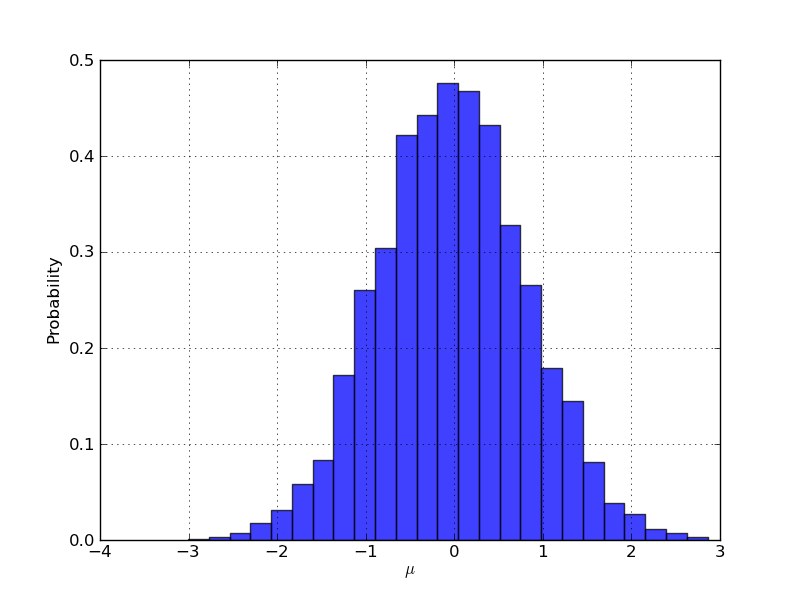
\includegraphics[width=3.5in]{figs/hist}
\end{center}

This matches quite well, and implies the basic kernel is functioning. Our next objective will be to 
move toward a few other distributions, with an eye on generating samples for a prior and posterior set of 
distributions that do not have an analytical solution. 

The codebase for this project has been developed on bitbucket, with logs
 for each commit. A fully functioning build system (a makefile) alongside a 'make  
 check' regression suite has been developed. At present, three
 regression tests are run, that perform simple checks on the
 distributions and sampling algorithm. The code has been tested on a local i7 quad core laptop, as well as TACC's
lonestar supercomputer. 

Finally, a directory, ``postprocessing'' contains scripts used to
generate all plots. These are routines using python with numpy+scipy and
matplotlib. 

\section{Future Work}

As mentioned in the previous section, the we will expand to a few other distributions, in addition to 
sampling gaussians. This should not be a significant part of the work. These distributions will also be 
verified against conjugate priors (analytically known solution distributions) when available. 

The largest remaining deliverable is to add OpenMP directives to the c++
implementation. Afterward, a detailed scaling study will be
performed. Due to the nature of MCMC, each markov chain should be
completely independent, and the underlying algorithm is therefore
``embarassingly parallel''. As a result, and we expect the routines to
scale essentially perfectly. At least, we hope so!

\end{document}
